\section{Badania}

W poniższym rozdziale przedstawione zostaną wyniki badań przeprowadzonych przez zespół w celu weryfikacji poprawności działania algorytmu Doc2Vec jako algorytmu umożliwiającego określenie podobieństwa pomiędzy artykułami. Opisane zostaną również zbiory danych uzyskane przez zespół na potrzeby testów.

\subsection{Znajdowanie artykułów podobnych jako zagadnienie klasyfikacji}

\par Uzyskanie wiarygodnej, liczbowej miary skuteczności znajdowania podobnych artykułów przez algorytm doc2vec wymagało formalnego zdefiniowania zagadnienia podlegającego ocenie. Zadanie to można zdefiniować jako zadanie klasyfikacji binarnej artykułów na dwie klasy: podobne i niepodobne.
\par Wymagało to przyjęcia pewnej definicji podobieństwa. Nastręczyło to zespołowi pewnej trudności. Na potrzeby oceny skuteczności algorytmów zespół przyjął podział zbiorów na dwie kategorie: artykułów identycznych oraz artykułów zbliżonych tematyką.
\par \textbf{Artykuły identyczne} określano jako artykuły, które traktują na temat dokładnie tego samego, konkretnego wydarzenia lub tej samej wypowiedzi danej osoby, jednak pochodzą z różnych źródeł lub w różnym czasie. Przykładem artykułów identycznych mogą być dwa artykuły o podjęciu decyzji o wspólnym występie reprezentacji obu Korei pod jedną flagą na Igrzyskach Olimpijskich w Pyeongchangu.
\par \textbf{Artykuły zbliżone} przyjęto jako artykuły dotyczące tej samej tematyki lub osoby, lecz nie mające wspólnej, konkretnej genezy - na przykład podzbiór artykułów o klubie piłkarskim Chelsea Londyn.
\par Wprowadzenie drugiej kategorii wymusiło na zespole zbudowanie sztucznego zbioru umożliwiającego ocenę możliwości rozpoznawania przez algorytm artykułów zbliżonych.
\par Zdefiniowanie podobieństwa pomiędzy artykułami umożliwiło etykietowanie par artykułów:
 \[c(x1, x2) = \begin{cases}
			0 & {x1, x2} - \text{niepodobne} \\
			1 & {x1, x2} - \text{podobne}
			\end{cases}
		\]
		
\par Formalnie, dalszej klasyfikacji podlegały więc nie same artykuły jako takie, lecz wygenerowane przez moduł analityczny podobieństwo pomiędzy parą artykułów:
$$ p(x1, x2), x1 \neq x2 - \text{Podobieństwo pomiędzy artykułami x1 i x2} $$
Podobieństwo to zostało wygenerowane jako iloczyn skalarny przeskalowanych wektorów dwóch artykułów. Ponieważ:
$$ p \in [0;1] $$
Podobieństwo to może być traktowane jako prawdopodobieństwo. Narzuca to analogię wyjścia modułu analitycznego jako klasyfikatora, zwracającego prawdopodobieństwo przynależności dwóch artykułów do klasy podobny. Zespół wykorzystał to do oceny skuteczności algorytmu porównywania artykułów w analogii do oceny klasyfikatora.

\subsection{Opis zbioru danych}

\par Na potrzeby przeprowadzenia badań zespół zbudował dwa zbiory artykułów. Zbiór roboczo nazwany ''rzeczywistym'' powstał przez faktycznne uruchomienie systemu agentowego i zbieranie artykułów z serwisów informacyjnych przez system bez względu na ich tematykę czy datę publikacji. Następnie były oceniane pod kątem podobieństwa tematyki i ręcznie etykietowane przez zespół. Zbiór sztuczny powstał poprzez odwrócenie takiego toku rozumowania - zamiast szukać w gotowym zbiorze podobnych artykułów, zespół wyszukiwał w internecie artykułów traktujących o identycznych bądź zbliżonych tematach.



\subsubsection{Zbiór rzeczywisty}

Zbiór rzeczywisty powstał poprzez uruchomienie gotowego systemu agentowego i pozyskanie artykułów z kanałów RSS następujących serwisów informacyjnych i mediów:
 
\begin{enumerate}
    \item CNN (29 artykułów)
    \item BBC (118 artykułów)
    \item The Guardian (81 artykułów)
    \item The New York Times (114 artykułów)
    \item Reuters (30 artykułów)
    \item The Washington Times (40 artykułów)
\end{enumerate}
 
Łącznie pobrano 412 artykułów. Dotyczyły one trzech zakresów tematycznych (\textit{tagów}):
\begin{enumerate}
	\item Science (70 artykułów)
	\item Technology (169 artykułów)
	\item Politics (173 artykuły)
\end{enumerate} 

Zespół zdecydował o utworzeniu zbioru klasyfikacyjnego na podstawie artykułów dotyczących tagu Politics. W procesie ręcznego przeglądania zbioru, zidentyfikowano łącznie 45 artykułów identycznych dotyczących 15 różnych tematów. W poniższej tabeli wymieniono tytuły, źródła i tematy artykułów identycznych ze zbioru.
 
\begin{center}
    \begin{longtable}{|p{.20\textwidth}|p{.40\textwidth}|p{.40\textwidth}|}
    \hline
    Serwis & Tytuł artykułu & Kategoria \\ \hline
    Reuters & Congress to vote Thursday for funding bill to avoid government shutdown & \multirow{5}{*}{Głosowanie w Kongresie} \\
    Washington Times & Donald Trump muscles in on GOP strategy to stop shutdown & \\ 
    Washington Times & James Lankford: Senate will use 'nuclear option' if his plan to limit debate time isn't passed & \\
    CNN & Republicans scramble to try to avert government shutdown as deadline nears & \\
    CNN & Government to shut down in 48 hours: What to watch & \\
    CNN & The Point: Republicans are going to get blamed for a government shutdown. Bigly. & \\ \hline
    Reuters & The Point: Republicans are going to get blamed for a government shutdown. Bigly. & \multirow{7}{*}{Przesłuchanie Bannona} \\
    Washington Times & Steve Bannon to be interviewed by Robert Mueller
& \\
    CNN & Axios: Bannon had a 'slip-up' in House Intelligence answer
 & \\
    CNN & Bannon's Hill appearance reveals White House effort to restrict testimony
 & \\
    CNN & Bannon will do interview with special counsel, avoiding grand jury for now
 & \\
    New York Times & North Korea, Bannon, Apple: Your Wednesday Evening Briefing
 & \\
    New York Times & Stephen Bannon, California, Bitcoin: Your Tuesday Evening Briefing
 & \\ \hline
 Reuters & Exclusive: Trump takes hard line on immigration, rejects 'horrible' bipartisan plan
 & \multirow{4}{*}{Ustawa imigracyjna Trumpa} \\
 Washington Times & White House official: Trump immigration views have evolved
 & \\
 CNN & McConnell:  Trump hasn't said what he wants in immigration bill 
& \\
 CNN & McConnell:  Trump hasn't said what he wants in immigration bill 
 & \\ \hline
 Washington Times & Kirstjen Nielsen: Democrats insult Border Patrol with focus on 's---hole' comment
 & \multirow{2}{*}{Komentarz Kristjen Nielsen} \\
 CNN & DHS Sec. Nielsen: 'I did not and will not lie under oath'
 & \\ \hline
 Guardian & & \multirow{3}{*}{Wspólny występ obu Korei na IO} \\
 New York Times & North and South Korean Teams to March as One at Olympics
 & \\
 New York Times & North Korean Orchestra Plans to Perform in South Korea During Winter Olympics
 & \\ \hline
 Guardian & Donald Trump's first year: in his own words - video
 & \multirow{3}{*}{Pierwszy rok Trumpa} \\
 CNN & Obama welcomed Trump to Washington a year ago. They haven't spoken since.
 & \\
 CNN & What we learned from 365 days of Trump polls
 & \\ \hline
 Guardian & Tillerson: US military to maintain open-ended presence in Syria – video
 & \multirow{2}{*}{Tillerson o Syrii} \\
 CNN & Tillerson's Syria wish list means US is in it for the longer haul 
 & \\ \hline
 Washington Times & Donald Trump insists the border wall will be built as promised & \multirow{2}{*}{Donald Trump o murze na granicy} \\
 CNN & After Kelly said Trump changed his 'attitude' on wall, Trump tweets it 'never changed'
 & \\ \hline
 CNN & John Kelly: Immigration 'hardass'
 & \multirow{2}{*}{Kelly o imigracji} \\
 CNN & Kelly on immigration: Trump 'has changed the way he's looked at a number of things'
 & \\ \hline
 Reuters & Exclusive: Trump accuses Russia of helping North Korea evade sanctions; says U.S. needs more missile defense
 & \multirow{3}{*}{Trump o Rosji i Korei} \\
 Guardian & Trump accuses Russia of violating sanctions to aid North Korea
 & \\
 CNN & Trump says 'Russia is not helping' with North Korea
 & \\ \hline
 New York Times & Sex Abuse Case Shadows Pope Francis’ Visit to Peru
 & \multirow{2}{*}{Wypowiedź Franciszka} \\
 New York Times & In Chile, Pope Francis Apologizes for ‘Irreparable Damage’ Caused by Sexual Abuse
 & \\ \hline
  New York Times & Suicide Bombers Attack Market in Nigeria, Killing at Least 12
 & \multirow{2}{*}{Zamach w Nigerii} \\
 New York Times & Gunmen Kidnap 2 Americans and 2 Canadians in Nigeria
 & \\ \hline
   New York Times & Facebook to Take Broader Look at Possible Russian Role in Brexit Vote
 & \multirow{2}{*}{Facebook o Brexicie} \\
 BBC & Facebook to reconsider claims of Russian interference in Brexit vote
 & \\ \hline
    New York Times & Days After Hawaii’s False Missile Alarm, a New One in Japan
 & \multirow{2}{*}{Fałszywy alarm na Hawajach} \\
 BBC & Warning system?
 & \\ \hline
 New York Times &  Carillion Collapse Could Lead to Thousands of Job Losses in U.K.
& \multirow{3}{*}{Carillion} \\
 BBC & Bonuses for Carillion bosses are blocked
 & \\
 BBC & Carillion's woes
 & \\ \hline
    \end{longtable}
\end{center}

Zbiór rzeczywisty został wyeksportowany z bazy danych i zapisany w postaci pliku csv do dalszej analizy.
Dla każdej pary artykułów ze zbioru rzeczywistego wygenerowano podobieństwo pomiędzy nimi. Ponieważ ocenie algorytmu podlega podobieństwo pomiędzy artykułami, utworzony zbiór miał:
\begin{enumerate}
	\item 56 par artykułów podobnych
	\item 14822 pary artykuł niepodobnych
\end{enumerate}

\subsubsection{Zbiór sztuczny}

Zbiór sztuczny został stworzony ręcznie przez twórców systemu i zawierał dwa rodzaje
artykułów. 
\begin{itemize}
\item artykuły identyczne - o tej samej tematyce,
\item artykuły zbliżone - o zbliżonej tematyce
\end{itemize}

Utworzono 3 grupy artykułów identycznych, każdy po 10 artykułów.
\begin{itemize}
\item sztorm w Holandii oraz Niemczech,
\item wyrzut cząsteczek z czarnej dziury,
\item podniesienie ceny serwisu Amazon Prime,
\end{itemize}

Artykułów o zbliżonej tematyce również powstały 3 grupy, również po 10 artykułów.
\begin{itemize}
\item wiadomości dotyczące Władimira Putina,
\item klub piłkarski Chelsea,
\item podatność Meltdown w procesorach Intel
\end{itemize}

\subsection{Miary oceny}

\par Zbiór utworzony na podstawie tagu Polityka zawiera zaledwie 56 pozycji o klasie 1 i niemal 15 000 pozycji o klasie 0. Jest to więc zbiór bardzo niezrównoważony. Właściwą metodą oceny algorytmów klasyfikacji dla takich zbiorów nie jest zatem dokładność klasyfikacji (co w opisywanym przypadku i tak nie miałoby sensu), lecz jej czułość i swoistość.
\par \textbf{Czułość} (ang. \textit{True Positive Rate}) należy w niniejszym projekcie zdefiniować jako zdolność wskazania klasy mniejszościowej - par artykułów podobnych.
\par \textbf{Swoistość} (ang. \textit{True Negative Rate}) należy zdefiniować jako zdolność poprawnego wskazania klasy większościowej - par artykułów niepodobnych.
\par Zaproponowana przez zespół analogia stopnia podobieństwa jako prawdopodobieństwa przynależności do klasy par artykułów podobnych nie daje jednak odpowiedzi binarnej. Należy ją uzyskać poprzez progowanie odpowiedzi modułu, uznając, iż jeśli podobieństwo jest powyżej określonego progu, to artykuły są podobne.
\par Najlepszą metodą oceny tego rodzaju algorytmu jest wykreślenie zależności pomiędzy czułością a swoistością dla wszystkich możliwych progów jako krzywej ROC (ang. \textit{Reverse Operating Characteristic}). Wobec tego wszystkie wyniki badań przeprowadzonych przez zespół będą poniżej opisane z wykorzystaniem tej krzywej.
\par Powszechnie wykorzystywaną miarą liczbową określającą poprawność działania algorytmu, którego wyniki są przedstawione na krzywej ROC, jest pole pod powierzchnią tej krzywej. Im bardziej zbliżone jest ono do wartości 1, tym lepszą klasyfikację algorytm umożliwia.


\subsection{Rezultaty}

\subsubsection{Badania na zbiorze sztucznym}

Badaniu podlegał zbiór par artykułów i podobieństwa pomiędzy nimi. Zbiór zawierał:
\begin{enumerate}
	\item 56 par artykułów podobnych
	\item 14822 pary artykuł niepodobnych
\end{enumerate}

\begin{figure}[H]
\centering
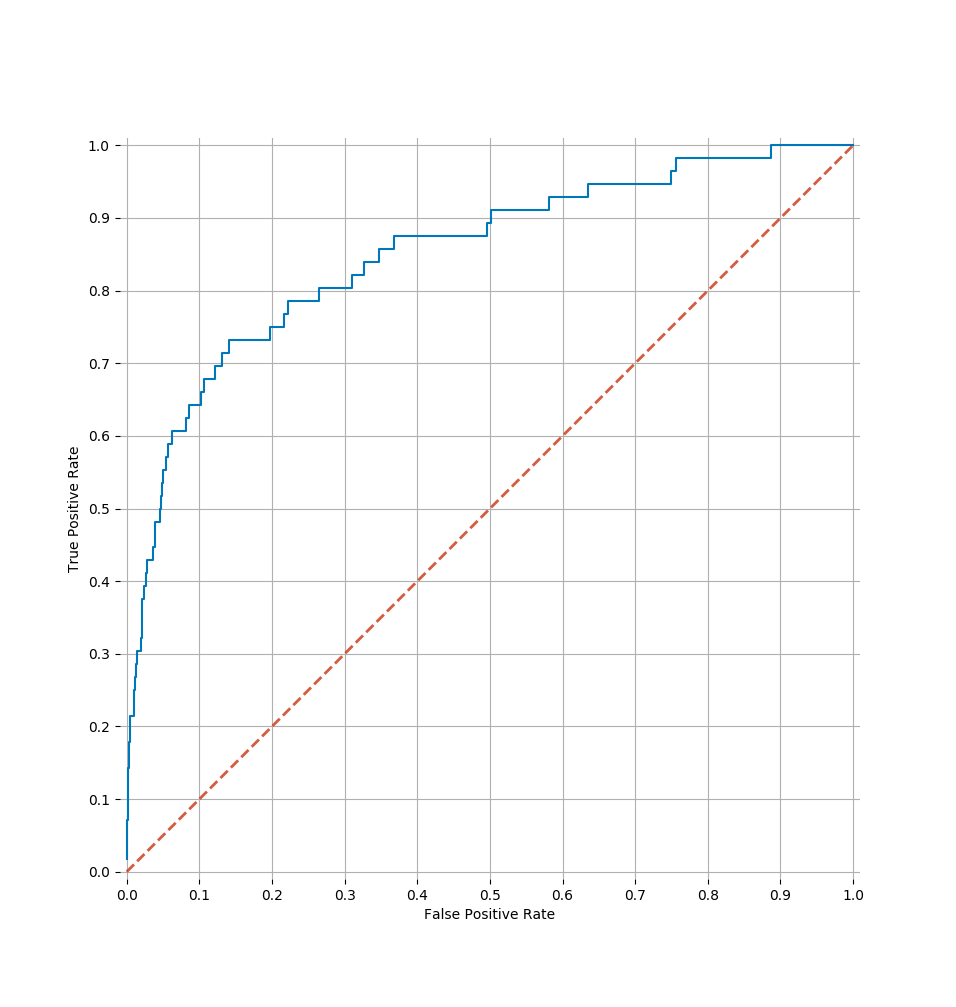
\includegraphics[width=0.8\textwidth]{./pict/roc_identical.png}
\caption{Krzywa ROC uzyskana na zbiorze rzeczywistym, AUC = 0.85}
\label{fig:rocidentical}
\end{figure}

Uzyskana krzywa ROC świadczy o tym, iż na rzeczywistym zbiorze artykułów algorytm bardzo dobrze radzi sobie z wskazywaniem artykułów o identycznej tematyce. Spośród 56 par artykułów podobnych, zaledwie 4 pary uzyskały stopień podobieństwa niższy niż średni stopień podobieństwa pomiędzy wszystkimi artykułami (0.3). Wszystkie pozostałe artykuły uzyskały znacząco wyższy stopień podobieństwa, co umożliwia dokonanie poprawnej klasyfikacji na podstawie progowania.



\subsubsection*{Artykuły źle klasyfikowane}

Celem znalezienia przyczyn niepowodzeń w klasyfikacji artykułów podobnych, zespół dokonał przeglądu par artykułów, których stopień podobieństwa uzyskany z modułu analitycznego jest niski.
\begin{enumerate}
	\item Pierwszą analizowaną parą artykułów są artykuły dotyczace wypowiedzi Rexa Tillersona na temat obecności Armii Stanów Zjednoczonych w Syrii:
	\begin{enumerate}
		\item CNN - Tillerson's Syria wish list means US is in it for the longer haul 
		\item Guardian - 
US military to maintain open-ended presence in Syria, Tillerson says
	\end{enumerate}
	Zespół upatruje przyczyny niepowodzenia w odmiennej naturze tych dwóch artykułów. Pierwszy spośród nich jest artykułem typowo opiniotwórczym, odnoszącym się do wypowiedzi Tillersona wyłącznie w kontekście Syrii, podczas gdy drugi z nich ma charakter relacji z wypowiedzi, pod koniec zaś odnosi się do posiedzenia Organizacji Narodów Zjednoczonych, czemu poświęcona jest niemal połowa artykułu.
	
	\item Druga niepodobna zdaniem algorytmu para artykułów dotyczy dwóch opiniotwórczych artykułow na temat pierwszego roku prezydentury Donalda Trumpa:
	\begin{enumerate}
		\item Donald Trump's first year: in his own words - video
		\item Obama welcomed Trump to Washington a year ago. They haven't spoken since.
	\end{enumerate}
	Przyczyna niepowodzenia okazała się oczywista po przejrzeniu pierwszego artykułu - jego treść jest w zasadzie wyłącznie nagłówkiem opatrującym nagranie zawierające wypowiedzi Trumpa, zaś same wypowiedzi nie są w nim transkryptowane.  Artykuły te dotyczą też tematyki pierwszego roku Trumpa, lecz w odniesieniu do różnych kwestii - drugi koncentruje się na relacji nowego prezydenta z poprzednim. Również kilka kolejnych pozycji spośród listy par artykułów tyczących się identycznej o najniższym stopniu podobieństwa zostało wygenerowanych jako porównania artykułu będącego zapowiedzią filmiku z innymi artykułami o pierwszym roku prezydentury.
\end{enumerate}

Analiza przypadków słabo sklasyfikowanych ujawniła ułomności uzyskanego zbioru, potwierdzając w gruncie rzeczy zdolności algorytmu do rozpoznawania artykułów podobnych.

\subsubsection*{Wyniki różnych modeli}
\label{sec:wyniki}

Jako podstawowy model, użyty został model trenowany na korpusie
Reutersa, i dla niego przeprowadzone zostały wszystkie powyższe
obliczenia. W wyniku pracy systemu udało się zgromadzić zbiór ok. 400
artykułów, który użyty został w celu uzyskania modelu o wyższej
dokładności. Eksperymenty te zostały opisane poniżej.


Wyniki modeli opisanych w sekcji \ref{ssec:modele} na sztucznym zbiorze
testowym, dla artykułów podobnych i zbliżonych:

\begin{center}
\begin{tabular}{r|c|c}
model & AUC -- podobny & AUC -- zbliżony\\
\hline
reuters & 0.9750 & 0.7047\\
reuters+rzeczywisty & 0.9893 & 0.8552\\
rzeczywisty & 1.0000 & 0.9000\\
\end{tabular}
\end{center}


\begin{figure}[p]
\centering
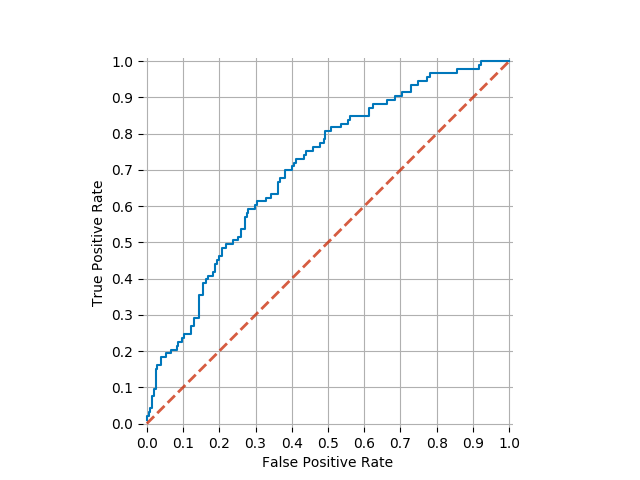
\includegraphics[width=0.8\textwidth]{./pict/reuters_z.png}
\caption{Krzywa ROC uzyskana na zbiorze testowym wiadomości zbliżonych  dla modelu trenowanego na korpusie Reuters, AUC = 0.7047}
\label{fig:rocidentical}
\end{figure}

\begin{figure}[p]
\centering
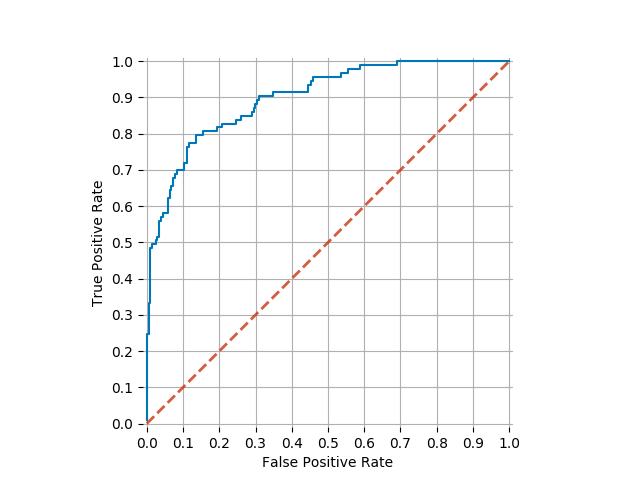
\includegraphics[width=0.8\textwidth]{./pict/dataset_z.png}
\caption{Krzywa ROC uzyskana na zbiorze testowym wiadomości zbliżonych dla modelu trenowanego na zbiorze rzeczywistym, AUC = 0.9000}
\label{fig:rocidentical}
\end{figure}

Z powyższych wyników można wysnuć dwa wnioski:

Po pierwsze, korpus wiadomości Reutersa jest zbyt różny od
rzeczywistego, aby jego użycie w treningu zwiększało wyniki
modelu. Zastąpienie go korpusem zbudowanym z wiadomości uzyskanych w
trakcie pracy systemu zwiększyło dokładność
klasyfikacji. Prawdopodobnie wynika to z różnicy w strukturze
wiadomości obu korpusów: korpus Reutersa zawiera, oprócz zwykłych
artykułów znaczną liczbę krótkich depeszy prasowych.

Po drugie, wiadomości dotyczące jednego konkretnego wydarzenia
(podobne) klasyfikowane są przez system dużo lepiej niż wiadomości
zbliżone (dotyczące różnych wydarzeń o podobnej tematyce). Jest to
oczekiwany wynik, świadczący o prawidłowym działaniu systemu.
